\documentclass[ENG]{fancynotes}
\usepackage[utf8]{inputenc}
\usepackage[T1]{fontenc}
\usepackage[english]{babel}
\usepackage{amsmath, amssymb, amsfonts}
\usepackage{geometry}
\usepackage{graphicx}
\usepackage{hyperref}
\usepackage{float}
\usepackage{lmodern}
\usepackage{tikz}
\usetikzlibrary{arrows.meta, positioning, calc}
\usepackage{setspace}
\setlength{\parindent}{0pt}
\geometry{a4paper, left=2.0cm, right=2.0cm, top=2.0cm, bottom=2.0cm}
\setstretch{1.1}

\title{\vspace{2em}Derivation of the Normal Form for a Three-Alternative Decision Model\\ (Based on Roxin, 2019) }
\author{F. Javier Rodríguez Martínez}
\date{}

\begin{document}
\maketitle

\section{Model and Expansion}

We consider the following system for three alternatives:
\begin{align}
  \tau\,\dot{r}_L &= -r_L + \phi\Bigl(s_L\,r_L - c\,r_I + I_L + U\Bigr) +\xi_L(t) ,  \label{eq:rL}\\[1mm]
  \tau\,\dot{r}_C &= -r_C + \phi\Bigl(s_C\,r_C - c\,r_I + I_C + U\Bigr)+\xi_C(t), \label{eq:rC}\\[1mm]
  \tau\,\dot{r}_R &= -r_R + \phi\Bigl(s_R\,r_R - c\,r_I + I_R + U\Bigr)+\xi_R(t), \label{eq:rR}\\[1mm]
  \tau_I\,\dot{r}_I &= -r_I + \phi_I\Bigl(\frac{g}{3}\bigl(r_L+r_R+r_C\bigr)+I_I\Bigr)+\xi_I(t). \label{eq:rI}
\end{align}

In a summarized form:

\begin{align}
  \tau\,\dot{r}_i &= -r_i + \phi\Bigl(s_i\,r_i - c\,r_I + I_i + U\Bigr)+\xi_i(t), \quad i=L,C,R, \label{eq:exc}\\[1mm]
  \tau_I\,\dot{r}_I &= -r_I + \phi_I\Bigl(\frac{g}{3}(R_L+R_C+R_R)+I_I\Bigr)+\xi_I(t), \label{eq:inh}
\end{align}
where:
\begin{itemize}
  \item \(r_i\) is the firing rate of excitatory population \(i\).
  \item \(r_I\) is the firing rate of the inhibitory population.
  \item \(s_i\) is the self-excitation coefficient (which may differ among populations).
  \item \(c\) is the inhibition coefficient.
  \item \(I_i\) are each population external input.
  \item \(U\) is a ramping urgency signal. We assume it varies slowly:
    \[
    U = U_0 + \varepsilon^2\,\Delta U.
    \]
	As U is a ramping signal, we have that $U_0 = 0$
  \item \(\tau\) and \(\tau_I\) are the time constants for the excitatory and inhibitory populations, respectively.
\end{itemize}

Our goal is to derive a reduced (normal form) model that captures the critical dynamics in a two-dimensional competitive subspace.

An schematic representation of the model is shown in figure \ref{fig:model-rates}.

\begin{figure}[H]
\centering
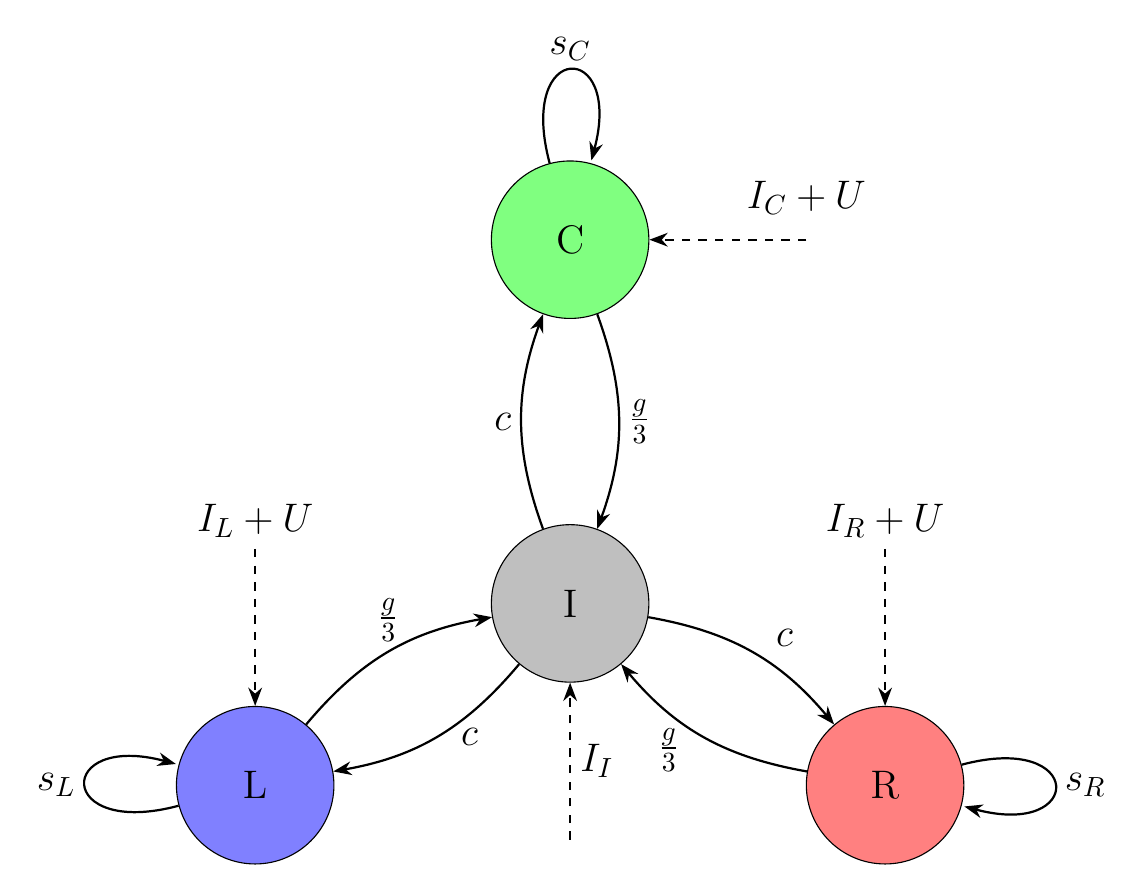
\begin{tikzpicture}[>=Stealth,
  neuron/.style={draw, circle, minimum size=2.0cm, inner sep=4pt, font=\Large},
  arrowlabel/.style={draw=none, fill=none, font=\Large}]

  % Define positions for the excitatory neurons (L, C, R)
  % For an equilateral triangle of side 8:
  % L at (-4, 0), R at (4, 0), C at (0, 6.928)
  \node[neuron, fill=blue!50] (L) at (-4,0) {L};
  \node[neuron, fill=green!50] (C) at (0,6.928) {C};
  \node[neuron, fill=red!50] (R) at (4,0) {R};
  
  % The inhibitory neuron (I) is placed at the centroid:
  % Centroid of triangle with vertices (-4,0), (4,0), (0,6.928) is at (0, (0+0+6.928)/3) = (0,2.309)
  \node[neuron, fill=gray!50] (I) at (0,2.309) {I};

  % Draw self-loops (representing self-excitation) for each excitatory neuron.
  \draw[->, thick] (L) edge[loop left] node[arrowlabel, left] {$s_L$} (L);
  \draw[->, thick] (C) edge[loop above] node[arrowlabel, above] {$s_C$} (C);
  \draw[->, thick] (R) edge[loop right] node[arrowlabel, right] {$s_R$} (R);

  % Draw connections from each excitatory neuron to the inhibitory neuron.
  \draw[->, thick, bend left=20] (L) edge node[arrowlabel, above] {$\tfrac{g}{3}$} (I);
  \draw[->, thick, bend left=20] (C) edge node[arrowlabel, right] {$\tfrac{g}{3}$} (I);
  \draw[->, thick, bend left=20] (R) edge node[arrowlabel, left, xshift = -5pt, yshift = -5pt] {$\tfrac{g}{3}$} (I);

  % Draw feedback connections from the inhibitory neuron to each excitatory neuron.
  \draw[->, thick, bend left=20] (I) edge node[arrowlabel, right, xshift = 5pt] {$c$} (L);
  \draw[->, thick, bend left=20] (I) edge node[arrowlabel, left] {$c$} (C);
  \draw[->, thick, bend left=20] (I) edge node[arrowlabel, right, xshift = 5pt, yshift = 5pt] {$c$} (R);

  % Draw external input arrows (dashed) to each excitatory neuron.
  \draw[->, dashed, thick] ($(L)+(0,3)$) -- (L) node[arrowlabel, pos = 0, yshift = 10pt ] {$I_L+U$};
  \draw[->, dashed, thick] ($(C)+(3,0)$) -- (C) node[arrowlabel, pos = 0, yshift = 15pt] {$I_C+U$};
  \draw[->, dashed, thick] ($(R)+(0,3)$) -- (R) node[arrowlabel, pos = 0, yshift = 10pt ]  {$I_R+U$};
  % Draw external input arrow to the inhibitory neuron.
  \draw[->, dashed, thick] ($(I)+(0,-3)$) -- (I) node[arrowlabel, midway, right] {$I_I$};

\end{tikzpicture}
\caption{Schematic representation of the rate model for 3-choice tasks. The choices are represented by three excitatory populations labeled L (Left), C (Center), and R (Right), which receive external inputs ($I_L$, $I_C$, and $I_R$, respectively) and exhibit self-excitation with strengths $s_L$, $s_C$, and $s_R$. There's also an external ramping input U common to all the excitatory populations. Each excitatory population affects to an inhibitory population (I) with weight $g/3$, and the inhibitory neuron provides feedback with strength $c$ to all excitatory populations. An external input $I_I$ is also applied to the inhibitory neuron.}
\label{fig:model-rates}
\end{figure}
\newpage


\subsection{Derivation of the normal form of order 2}
\subsubsection{Expansion of the system}
We assume a series expansion for the solution:
\begin{align}
  r_i(t) &= R_i + \varepsilon\,r_{1,i}(t) + \varepsilon^2\,r_{2,i}(t) + O(\varepsilon^3), \quad i=L,C,R, \label{eq:exp_ex}\\[1mm]
  r_I(t) &= R_I + \varepsilon\,r_{1,I}(t) + \varepsilon^2\,r_{2,I}(t) + O(\varepsilon^3). \label{eq:exp_inh}
\end{align}


We will also consider variations of s,  $s = s_0 +\varepsilon^2 \bar{s_i} + O(\varepsilon^3)$. 
Thus, the fixed point \(R=(R,R,R,R_I)\) is determined at \(O(1)\):
\begin{align}
  R &= \phi\Bigl(s_0\,R - c\,R_I + I_0  \Bigr), \quad i=L,C,R, \label{eq:fixed_ex}\\[1mm]
  R_I &= \phi_I\Bigl({g}R+I_I\Bigr). \label{eq:fixed_inh}
\end{align}

Additionally, we introduce a slow time scale:
\[
T = \varepsilon\,t,
\]
so that
\[
\frac{d}{dt} = \frac{\partial}{\partial t} + \varepsilon\,\frac{\partial}{\partial T}.
\]


We define
\begin{equation}
  X_i = s_i\,r_i - c\,r_I + I_i + U.
  \label{eq:argument}
\end{equation}
Substituting the expansions:
\[
X_i = (s_0+ \varepsilon^2 \bar{s}_i)\,(R + \varepsilon\,r_{1,i} +\varepsilon^2 r_{2,i} \cdots) - c\,(R_I + \varepsilon\,r_{1,I}+\varepsilon^2 r_{2,i} +\cdots) + I_0 +\varepsilon^2 \bar{I}_i + U_0 + \varepsilon^2\,\Delta U.
\]
We then group:
\begin{itemize}
  \item Order \(O(1)\):
    \[
X_0 = s_0 R - c R_I +I_0 + U_0
    \]
  \item Order \(O(\varepsilon)\):
    \[
   X_{i,1} = \varepsilon [s_0 r_{1,i}- cr_{1,I}]
    \]
  \item Order \(O(\varepsilon^2)\): 
\[
X_{i,2} = \varepsilon^2 [s_0 r_{2,i}+ R\bar{s_i} + \Delta U + \bar{I_i}]
\]
  \item Order \(O(\varepsilon^3)\): 
\[
X_{i,3} = \varepsilon^3 [s_0 r_{3,i}+ r_{1,i}\bar{s_i}]
\]
\end{itemize}






The Taylor expansion of \(\phi\) about \(X_{i,0}\) is
\begin{equation}
\phi(X_i) = \phi(X_0) + \phi'(X_0) (\Delta X_i) + \frac{1}{2}\,\phi''(X_0) (\Delta X_i)^2 +\frac{1}{6}\,\phi'''(X_0) (\Delta X_i)^3+ O(\varepsilon^4)
\label{eq:taylor_exp}
\end{equation}
with
\[
\Delta X_i = \varepsilon [s_0 r_{1,i}- cr_{1,I}] + \varepsilon^2[R\bar{s}_i + \Delta U + \bar{I}] + O(\varepsilon^3)
\]


From this point on, we will exclude the dependence of $\phi(X)$ and it's derivatives and write them as $\phi, \phi'...$


For the equation (\ref{eq:exc}), substituting the expansion we have:


At \(O(1)\):
\[
R = \phi(X_{0}), \quad i=L,C,R.
\]
The \textbf{bifurcation condition} we impose is:
\begin{equation}
  s_0\,\phi'(X_{0}) = 1, \quad i=L,C,R.
  \label{eq:bifurcation_condition}
\end{equation}


Thus, at \(O(\varepsilon)\):
\[
\tau \dot{r}_{1,i} = \underbrace{(-1+s_{0} \phi'(X_0))}_0 r_{1,i} - c\phi'(X_0)r_{1,I}
\]




Similarly, linearizing the inhibitory equation (\ref{eq:inh}) gives:
\begin{equation}
  \tau_I\,\dot{r}_{1,I} = -r_{1,I} + \phi_I'\Bigl(\frac{g}{3}(r_{L,1}+r_{C,1}+r_{R,1})+I_I\Bigr)\sum_{i=L,C,R}r_{i,1}.
  \label{eq:order1_inhibitory}
\end{equation}

The eigenvectors for the underlying DM process can be found solving:
\[
L_0\,r_1 = 0,
\]
with

\[ 
  L_0 = \begin{pmatrix}
    0 & 0 & 0 & c\,\phi' \\[2mm]
    0 & 0 & 0 & c\,\phi' \\[2mm]
    0 & 0 & 0 & c\,\phi' \\[2mm]
    -\dfrac{g}{3}\,\phi_I' & -\dfrac{g}{3}\,\phi_I' & -\dfrac{g}{3}\,\phi_I' & 1
  \end{pmatrix}.
  \label{eq:L0_matrix}
\]


\bigskip

Due to the slow time scale \(T=\varepsilon\,t\), the time derivative expands as:
\[
\frac{d}{dt} = \frac{\partial}{\partial t} + \varepsilon\,\frac{\partial}{\partial T}.
\]


The order \(\varepsilon^2\) equation is written as
\begin{equation}
  L_0\,r_2 + L_1\,r_1 = N_2,
  \label{eq:order2_eq}
\end{equation}

Where,

\begin{equation}
  L_1 = \begin{pmatrix}
    \tau\,\partial_T & 0 & 0 & 0 \\[2mm]
    0 & \tau\,\partial_T & 0 & 0 \\[2mm]
    0 & 0 & \tau\,\partial_T & 0 \\[2mm]
    0 & 0 & 0 & \tau_I\,\partial_T
  \end{pmatrix}.
  \label{eq:L1_matrix}
\end{equation}

\bigskip


To compute $N_2$ we make use of the Taylor formula (\ref{eq:taylor_exp}):
\begin{equation}
\phi(X_i) = \phi(X_0) + \varepsilon \phi'(X_0) (s_0r_{1,i}-cr_{1,I}) +\varepsilon^2\left(\phi'(X_0)(R\bar{s_i} + \Delta U +\bar{I_i}) + \frac{1}{2}\,\phi''(X_0)  (s_0r_{1,i}-cr_{1,I})^2\right) + O(\varepsilon^3)
  \label{eq:taylor_full2}
\end{equation}


Then,
\begin{equation}
N_2 = \phi'\begin{pmatrix}
\bar{I}_L + R\bar{s}_L +\Delta U  \\\bar{I}_C  + R\bar{s}_C +\Delta U\\ 
\bar{I}_R + R\bar{s}_R +\Delta U\\ 
0
\end{pmatrix} + \frac{1}{2} 
\begin{pmatrix}\phi'' (s_0r_{L,1} - cr_{1,I})^2\\  
\phi''(s_0r_{C,1} - cr_{1,I})^2\\  
\phi''(s_0r_{R,1} - cr_{1,I})^2 \\ 
\phi''_I \frac{g^2}{9}(r_{L,1} +r_{C,1} + r_{R,1}) 
\end{pmatrix}
\label{eq:N2}
\end{equation}


Since \(L_0\) has a nontrivial null space (by the bifurcation condition), we can write the solution of $L_0r_1 = 0$  in terms of a basis of this null space, for example, we choose:
\[
e_1 = (1, -1, 0, 0), \quad e_1 = (1, 1, -2, 0).
\]

Thus, the $O(\varepsilon)$ solution can be written as:
\[
r_1 = e_1\,X_1(T) + e_2\,X_2(T),
\]
Where $X_1 = r_L-r_C, X_2 =  r_L+r_C-2r_R, $

In consequence, we have that:
 \[
r_{1} = \begin{pmatrix}X_1+X_2\\-X_1+X_2\\-2X_2\\0 \end{pmatrix} 
\]


We can now rewrite $N_2$ in terms of $X_1, X_2$ as:

\[
N_2 = \phi'\begin{pmatrix}
\bar{I}_L + R\bar{s}_L +\Delta U  \\\bar{I}_C  + R\bar{s}_C +\Delta U\\ 
\bar{I}_R + R\bar{s}_R +\Delta U\\ 
0
\end{pmatrix} + \frac{s_0^2 \phi''}{2} 
\begin{pmatrix}
(X_1 +X_2)^2\\  
(-X_1 + X_2)^2\\  
4X_2^2\\ 
0
\end{pmatrix}
\]

\subsubsection{Solvability conditions}
If we multiply by a vector  $v^T  \in ker(L_0)$, we obtain:

$$
v^T N_2 = \underbrace{v^T L_0 r_1}_0 + v^T L_1 r_0 = v^T L_1 r_0
$$
Thus, 
$$
v^T N_2 - v^T L_1 r_0 = 0 \implies \langle v^T,  N_2 - L_1 r_0\rangle = 0 \implies \langle v^T,  N_2 \rangle = 0 
$$

In consequence, our solvability conditions will be:
\begin{equation}
\begin{aligned}
    \langle e_1, L_1 r_1 \rangle &= \langle e_1, N_2 \rangle \\
    \langle e_2, L_1 r_1 \rangle &= \langle e_2, N_2 \rangle
\end{aligned}
 \label{eq:solvability1}
\end{equation}

This results in the \textbf{second order normal form} equations:
\begin{equation}
\begin{aligned}
\tau \dot{X}_1 &= \frac{\phi'}{2}(\bar{I}_L -  \bar{I}_C + R (\bar{s}_L - \bar{s}_C)) + s_0^2\phi''(X_1X_2) + \frac{1}{2}(\xi_L(t)-\xi_C(t)) \\[8pt]
\tau \dot{X}_2 &= \frac{\phi'}{6}(\bar{I}_L +  \bar{I}_C - 2 \bar{I}_R +  R (\bar{s}_L+ \bar{s}_C -2\bar{s}_R) ) + \frac{s_0^2\phi''}{6}(X_1^2-3X_2^2) + \frac{1}{6}(\xi_L(t)+\xi_C(t)-2\xi_R(t))
\end{aligned}
\label{eq:secondorder}
\end{equation}

\subsubsection{Potential derivation}

We can think of this equations as the field in $\mathbb{R}^2$, $F(X_1,X_2) = (F_1,F_2) =(\bar{F_1},\bar{3F_2})$, where 
\begin{align*}
\bar{F_1} &=  \frac{\phi'}{2}(\bar{I}_L -  \bar{I}_C + R(\bar{s}_L - \bar{s}_C)) + s_0^2\phi''(X_1X_2)\\
\bar{F_2} &= \frac{\phi'}{6}(\bar{I}_L +  \bar{I}_C - 2 \bar{I}_R + R(\bar{s}_L+ \bar{s}_C -2\bar{s}_R)) + \frac{s_0^2\phi''}{6}(X_1^2-3X_2^2) 
\end{align*}


The field defined by this equations is irrotational as:
\begin{equation}
\begin{aligned}
 \frac{\partial \bar{F_1}}{\partial y}& = X_{1} \phi{''} s_{0}^{2} \\[8pt]
 \frac{\partial\bar{ F_2}}{\partial x} & = \frac{X_{1} \phi{''} s_{0}^{2}}{3} 
\end{aligned}
\label{eq:secondorder}
\end{equation}

In consequence, it exists a potential $\psi$ such that $\frac{\partial \psi}{\partial x} = F_1, \frac{\partial \psi}{\partial y} = F_2 $:
\[
\psi(X_1,X_2) = \frac{1}{2}( X_{1}^{2} X_{2} \phi'' s_{0}^{2} - X_{1} \phi' \left(I_C - I_L +R  (s_C - s_L)\right)- X_{2}^{3} \phi'' s_{0}^{2} + X_{2} \phi' \left(I_C + I_L - 2 I_R + R(s_C + s_L - 2 s_R)\right))
\]

\begin{figure}[H]
\begin{center}
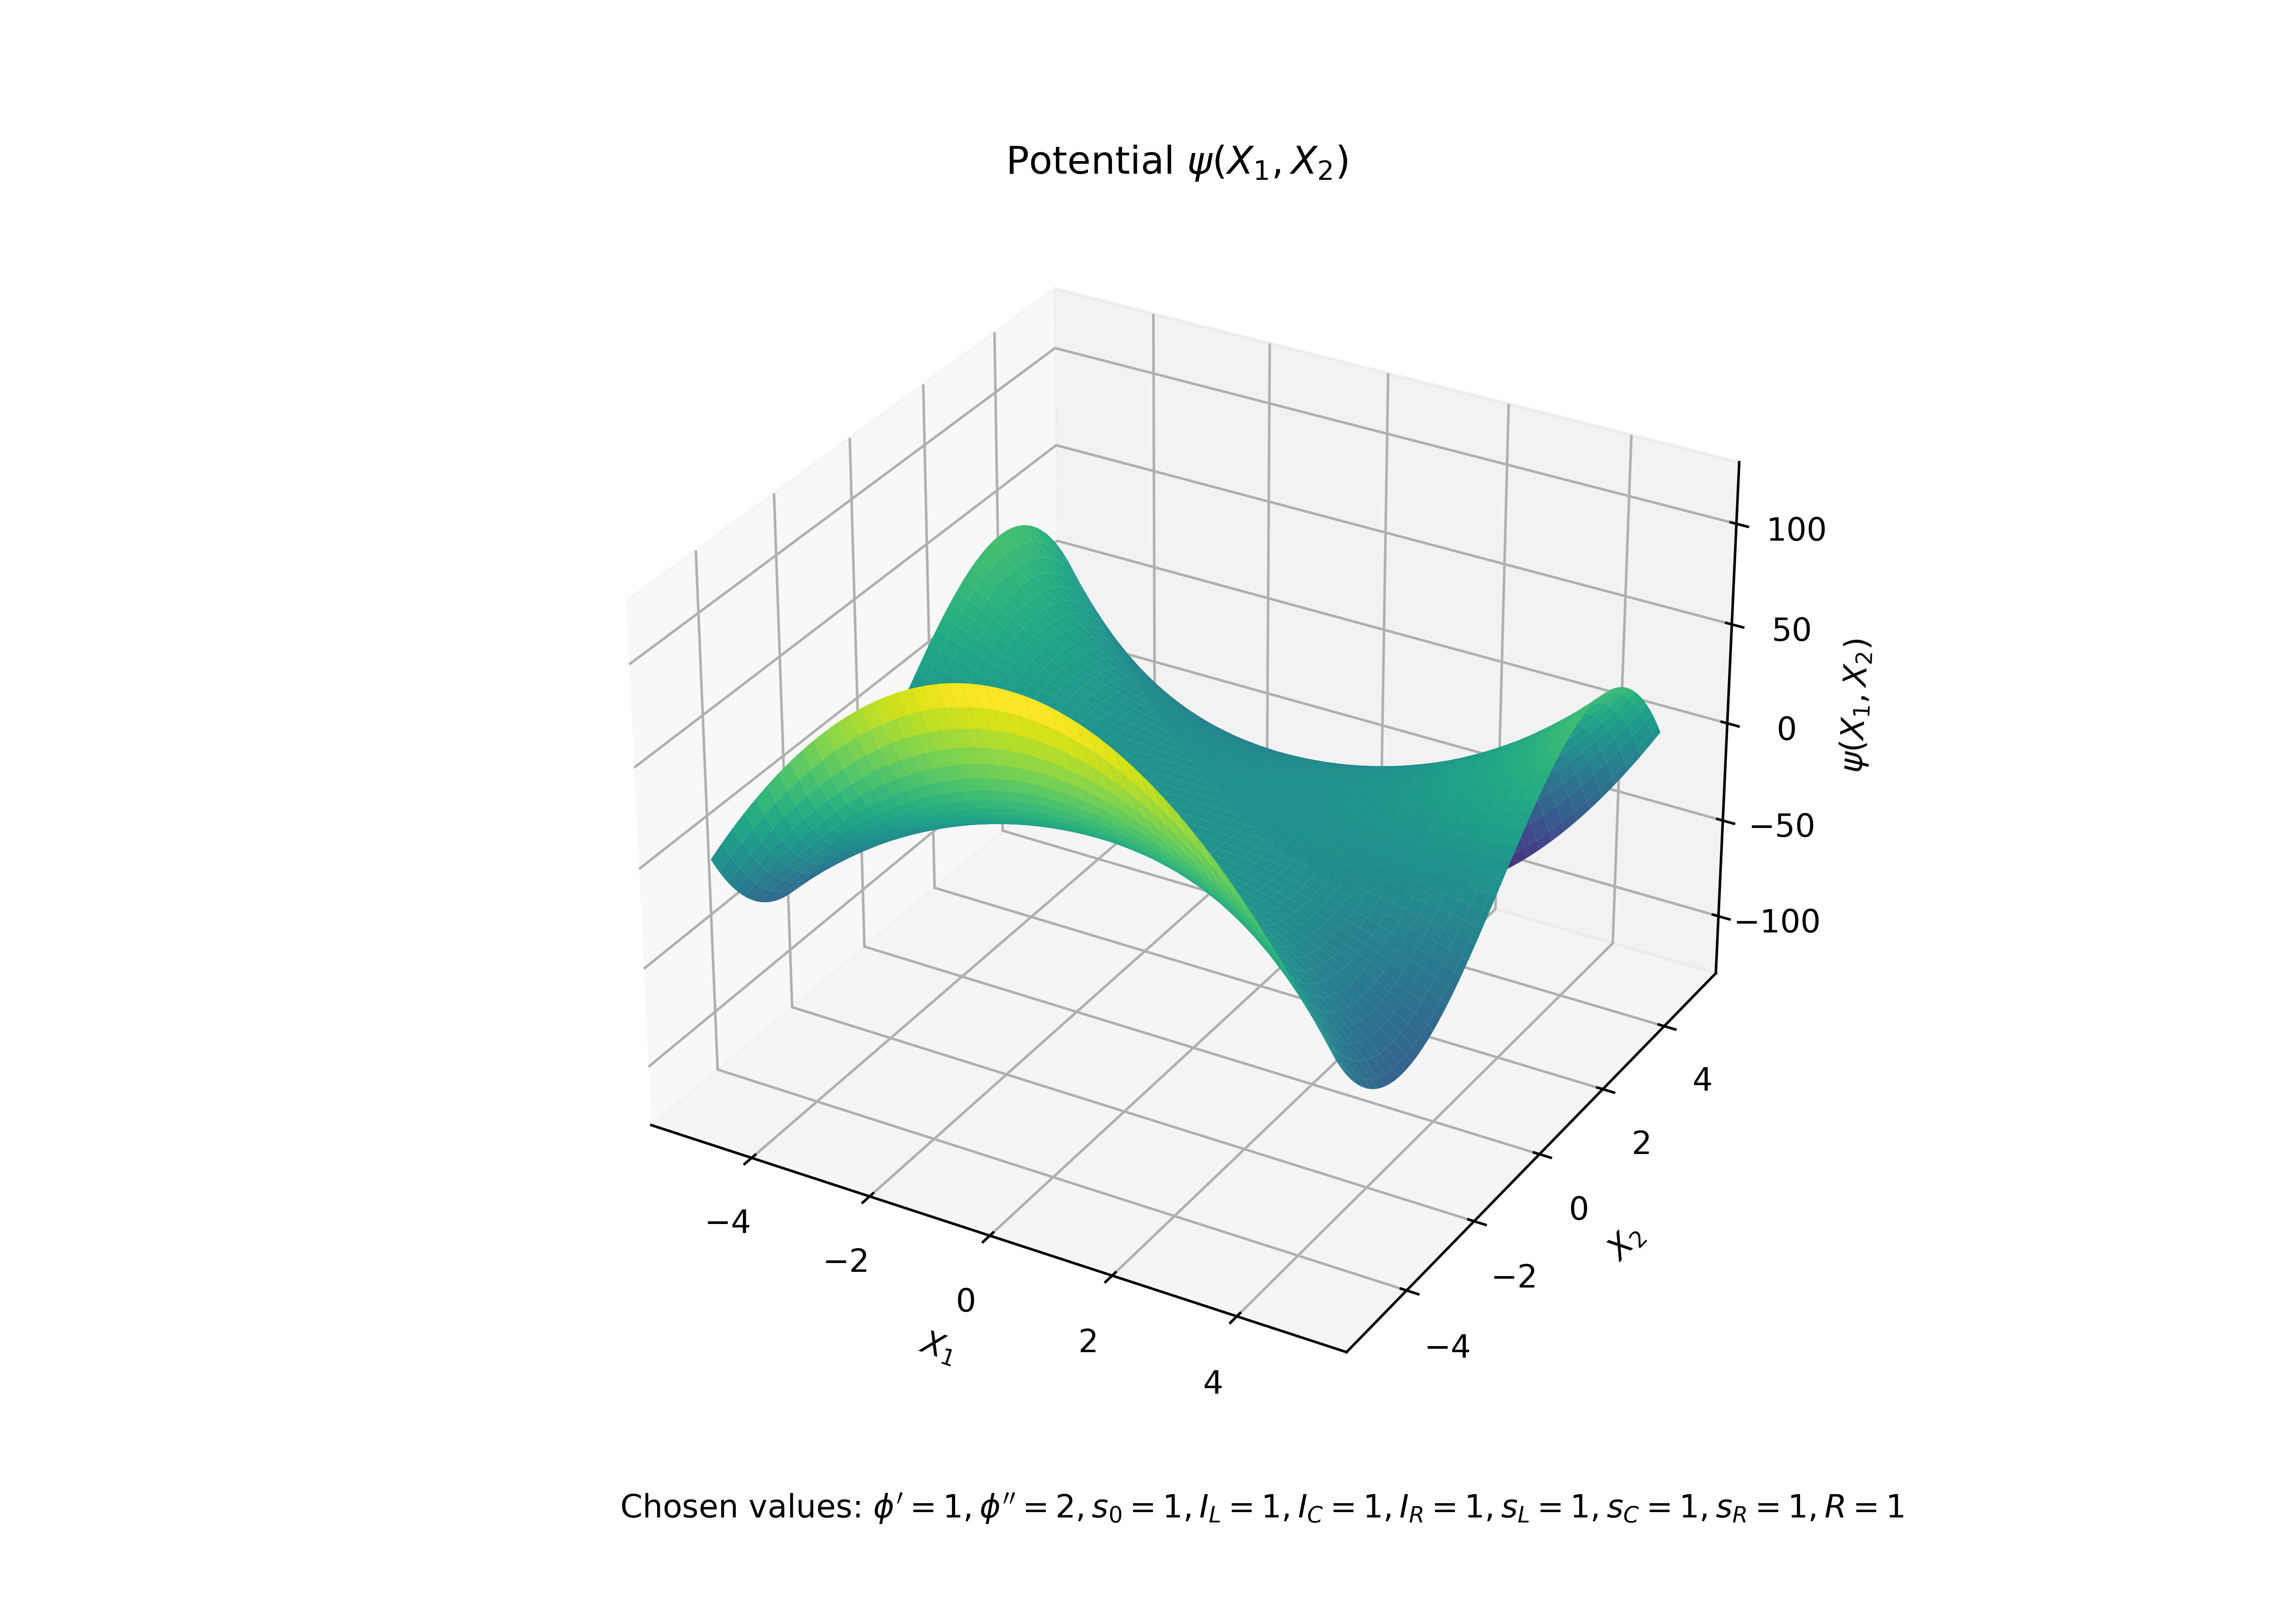
\includegraphics[width = 0.9\textwidth]{plots/potencial.png}
\caption{Potential obtained from the order 2 normal equations.}
\end{center}
\end{figure}

\subsection{Derivation of the normal form of order 3}

We can go up to third order to obtain more terms in this potential:

Now, $r_2$ has components in the directions $e_c = \begin{pmatrix}
1,1,1,0\\
\end{pmatrix}$ and $e_I = \begin{pmatrix}0,0,0,1\\\end{pmatrix}$. 

Taking $r_2 = e_CR_{2C} + e_IR_{2I}$ :

 \[
r_{2} = \begin{pmatrix}R_{2C}\\R_{2C}\\R_{2C}\\R_{2I} \end{pmatrix} 
\]


Projecting the equations:

\begin{equation}
\begin{aligned}
\langle e_c , L_0r_2 \rangle = \langle e_c, N_2\rangle\\[8pt]
\langle e_I , L_0r_2 \rangle = \langle e_I, N_2\rangle
\end{aligned}
\label{eq:secondorder}
\end{equation}

Then as, \[L_0r_2 = \begin{pmatrix}
c\phi'R_{2I},c\phi'R_{2I},c\phi'R_{2I}, -g\phi'_IR_{2C} +R_{2I}\\
\end{pmatrix}\]

We obtain the system of equations:
%
%\begin{pmatrix}
%(X_1 -X_2)^2\\  
%(-X_1 + X_2)^2\\  
%4X_2^2\\ 
%0
%\end{pmatrix}

\begin{equation}
\begin{aligned}
3c\phi'R_{2I}  &= \phi'(\bar{I}_L+\bar{I}_C+\bar{I}_R + R(\bar{s}_L+ \bar{s}_C+ \bar{s}_R) +3\Delta U )+ \frac{s_0^2\phi''}{2}\left(2X_1^2+6X_2^2 \right)\\[8pt]
-g\phi'R_{2C} +R_{2I} &= 0
\end{aligned}
\label{eq:}
\end{equation}


Isolating, we find:
\[
R_{2C} = \frac{1}{g\phi'_I}R_{2I} \qquad R_{2I} = \frac{1}{3c}(\bar{I}_L+\bar{I}_C+\bar{I}_R + R(\bar{s}_L+ \bar{s}_C+ \bar{s}_R) +3\Delta U )+ \frac{s_0^2\phi''}{3c\phi'}(X_1^2+3X_2^2)
\]

Including $r_2$ and the terms O($\varepsilon^3$) in $\Delta X_i$:
\begin{equation}
\Delta X_i = \varepsilon [s_0 r_{1,i}- cr_{1,I}] + \varepsilon^2[R\bar{s}_i + s_0r_{2,i} - c r_{2,I}+ \Delta U + \bar{I}] + \varepsilon^3 [r_{1,i}\bar{s_i} ]
\end{equation}
% Porque no incluye s_0 r_{3,i}

The $O(\varepsilon^3)$ term in the Taylor expansion of $\phi(X_i)$ is:
\begin{equation}
\varepsilon^3\left(\phi'(r_{1,i}\bar{s_i}) +\phi''(s_o r_{1,i}-cr_{1,I})(R\bar{s_i}+ s_0r_{2,i} - c r_{2,I}+ \Delta U + \bar{I_i}) + \frac{1}{6} \phi'''(s_o r_{1,i}-cr_{1,I})^3  \right) 
\end{equation}

Now, the equations up to $O(\varepsilon^3)$ are:
\[
L_0r_3 + L _{1} r_{2} = N _{3}
\]


Where, 
\[
N_3 = 
\phi'\begin{pmatrix}
\bar{s}_L(X_1+X_2)\\
\bar{s}_C(-X_1+X_2)\\ 
\bar{s}_R(-2X_2)\\ 
0
\end{pmatrix} +\phi''s_0\begin{pmatrix}
(X_1+X_2)(R\bar{s_L} + \underbrace{s_0R_{2C} - cR_{2I}}_{(s_0-cg\phi'_I)R_{2C}}+ \Delta U + \bar{I}_L)\\
(-X_1+X_2)(R\bar{s_C} +(s_0-cg\phi'_I)R_{2C}+ \Delta U + \bar{I}_C)\\ 
(-2X_2)(R\bar{s_R} +(s_0-cg\phi'_I)R_{2C}+ \Delta U + \bar{I}_R)\\ 
0
\end{pmatrix} + \frac{\phi'''s_0^3}{6} 
\begin{pmatrix}
(X_1 + X_2)^3\\  
(-X_1 + X_2)^3\\  
-8X_2^3 \\ 
 0
\end{pmatrix}
\]

Applying the solvability conditions, we obtain the equations:
\begin{equation}
0 = \langle e_1, N_3\rangle \quad 0 = \langle e_2, N_3 \rangle
\end{equation}

Solving, we can add this terms to the second order normal form and obtain the \textbf{third order normal form} equations: 
\begin{equation}
\begin{aligned}
0 = & \; \phi'(X_1(\bar{s}_L+ \bar{s}_C)+X_2(\bar{s}_L -\bar{s}_C))\\
&+ s_0 \phi'' \Bigl( X_1(R(\bar{s}_L+\bar{s}_C)+2(s_0-cg\phi'_I)R_{2C}  + 2\Delta U + \bar{I}_L + \bar{I}_C) \Bigr) + X_2\bigl(R(\bar{s}_L-\bar{s}_C) + \bar{I}_L - \bar{I}_C\bigr)\\
&+ \frac{\phi'''s_0^3}{3}  X_1\bigl(X_1^2+3X_2^2\bigr)
\end{aligned}
\end{equation}

\begin{equation}
\begin{aligned}
0 = &\; \phi'(X_1(\bar{s}_L- \bar{s}_C)+X_2(\bar{s}_L +\bar{s}_C+4\bar{s}_R))\\ 
& + s_0\phi'' \Bigl(X_1(R(\bar{s}_L-\bar{s}_C) + \bar{I}_L - \bar{I}_C) + X_2(R(\bar{s}_L+\bar{s}_C+ 4\bar{s}_R)+ 6(s_0-cg\phi'_I)R_{2C}  + 6\Delta U+ (\bar{I}_L + \bar{I}_C + 4\bar{I}_R))\Bigr)\\
&+ \phi'''s_0^3 X_2\bigl(X_1^2+3X_2^2\bigr)
\end{aligned}
\end{equation}




\end{document}
